

%%
%% forked from https://gits-15.sys.kth.se/giampi/kthlatex kthlatex-0.2rc4 on 2020-02-13
%% expanded upon by Gerald Q. Maguire Jr.
%% This template has been adapted by Anders Sjögren to the University
%% Engineering Program in Computer Science at KTH ICT. Adaptation is the
%% translation of English headings into Swedish as the addition of Swedish
%% text. Original body text is deliberately left in English.

%% Conventions for todo notes:
% \todo[inline]{Comments/directions/... in English}
% \todo[inline, backgroundcolor=kth-lightblue]{Text på svenska}
% \todo[inline, backgroundcolor=kth-lightgreen]{English descriptions about formatting}

%% The template is designed to handle a thesis in English or Swedish
% set the default language to english or swedish by passing an option to the documentclass - this handles the inside tile page
% To optimize for digital output (this changes the color palette add the option: digitaloutput
% To use bibtex or biblatex - include one of these as an option
\documentclass[english, bibtex]{kththesis}
%\documentclass[swedish, biblatex]{kththesis}

% \usepackage[style=numeric,sorting=none,backend=biber]{biblatex}
\ifbiblatex
    %\usepackage[language=english,bibstyle=authoryear,citestyle=authoryear, maxbibnames=99]{biblatex}
     \usepackage[bibstyle=authoryear,citestyle=authoryear, maxbibnames=99,language=english]{biblatex}
    \addbibresource{references.bib}
\else
    % The line(s) below are for BibTeX
    \bibliographystyle{bibstyle/myIEEEtran}
    %\bibliographystyle{apalike}
\fi


% include a variety of packages that are useful
%%%%%%%%%%%%%%%%%%%%%%%%%%%%%% Packages %%%%%%%%%%%%%%%%%%%%%%%%%%%%%%
%% The following are needed for generating the DiVA page(s)
\usepackage{scontents}              %% Needed to save lang, abstract, and keywords
\usepackage{pgffor}                 %% includes the foreach loop

%% Basic packages

%% Links
\usepackage{url}                %% Support for breaking URLs

%% Colorize
%\usepackage{color}
\PassOptionsToPackage{dvipsnames, svgnames}{xcolor}
\usepackage{xcolor}

\usepackage[normalem]{ulem}
\usepackage{soul}
\usepackage{xspace}
\usepackage{braket}

% to support units and decimal aligned columns in tables
% the option loads the binary prefixes
\usepackage[binary-units=true, locale=US]{siunitx}

\usepackage{balance}
\usepackage{stmaryrd}
\usepackage{booktabs}
\usepackage{graphicx}	        %% Support for images
\usepackage{multirow}	        %% Support for multirow columns in tables
\usepackage{tabularx}		    %% For simple table stretching
\usepackage{mathtools}
\usepackage{algorithm} 
\usepackage{algorithmic}  
\usepackage{amsmath}
\usepackage[linesnumbered,ruled,vlined,algo2e]{algorithm2e}
% can't use both algpseudocode and algorithmic packages
%\usepackage[noend]{algpseudocode}
%\usepackage{subfig}  %% cannot use both subcaption and subfig packages
\usepackage{optidef}
\usepackage{float}		        %% Support for more flexible floating box positioning
\usepackage{pifont}

%% some additional useful packages
% to enable rotated figures
\usepackage{rotating}	    	%% For text rotating
\usepackage{array}		        %% For table wrapping
\usepackage{mdwlist}            %% various list-related commands
\usepackage{setspace}           %% For fine-grained control over line spacing


\usepackage{enumitem}           %% to allow changes to the margins of descriptions


%% If you are going to include source code (or code snippets)
\usepackage{listings}		    %% For source code listing
%%\usepackage[cache=false]{minted} %% For source code highlighting
%%\usemintedstyle{borland}

\usepackage{bytefield}          %% For packet drawings


\setlength {\marginparwidth }{2cm} %leave some extra space for todo notes
\usepackage{todonotes}
\usepackage{notoccite} % do not number captions based on their appearance in the TOC


% Footnotes
\usepackage{perpage}
\usepackage[perpage,para,symbol]{footmisc} %% use symbols to ``number'' footnotes and reset which symbol is used first on each page


%% Various useful packages
%%----------------------------------------------------------------------------
%%   pcap2tex stuff
%%----------------------------------------------------------------------------
\usepackage{tikz}
\usetikzlibrary{arrows,decorations.pathmorphing,backgrounds,fit,positioning,calc,shapes}
\usepackage{pgfmath}	% --math engine
\newcommand\bmmax{2}
\usepackage{bm} % bold math


%% Managing titles
% \usepackage[outermarks]{titlesec}
%%%%%%%%%%%%%%%%%%%%%%%%%%%%%%%%%%%%%%%%%%%%%%%%%%%%%%%%%%%%%%%%%%%%%%
%\captionsetup[subfloat]{listofformat=parens}

% to include PDF pages
%\usepackage{pdfpages}


\usepackage{csquotes}               %% Recommended by biblatex
% to provide a float barrier use:
\usepackage{placeins}

\usepackage{comment}  %% Provides a comment environment




%%% Local Variables:
%%% mode: latex
%%% TeX-master: t
%%% End:
% KTH colors for LaTeX documents
%
% Started from kthcolors by:
% Riccardo Sven Risuleo
% 2016-09-06 11:05:40
%
% from https://github.com/KTH-AC/kthcolors
%
% Adapted using the colors from "Graphic Profile Manual KTH" version 180604
% (i.e.. 2018-06-04) 
% see https://intra.kth.se/en/administration/kommunikation/grafiskprofil/kth-s-grafiska-profil-1.844676
% 
% G. Q. Maguire Jr.
% 2021-07-05
%

%\NeedsTexFormat{LaTeX2e}[1994/06/01]
%\ProvidesPackage{kthcolors}[2021/07/85 v3 Latex package with official KTH colors]

\RequirePackage{xcolor}
%% Primary colors
%% As of the new manual, there is only 1 primary color; but with three 
\definecolor{kth-blue}{RGB/cmyk}{25,84,166/0.849,0.494,0,0.349}
\colorlet{kth-blue80}{kth-blue!80!}
\colorlet{kth-blue40}{kth-blue!40!}

% these are no longer used as of 2018-06-04
%\definecolor{kth-red}{RGB/cmyk}{157,16,45/0,0.898,0.713,0.384}
%\definecolor{kth-green}{RGB/cmyk}{98,146,46/0.329,0,0.685,0.427}

%% Secondary colors
\definecolor{kth-lightblue}{RGB/cmyk}{36,160,216/0.833,0.259,0,0.153}
\colorlet{kth-lightblue80}{kth-lightblue!80!}
\colorlet{kth-lightblue40}{kth-lightblue!40!}

%\definecolor{kth-lightred}{RGB/cmyk}{228,54,62/0,0.763,0.728,0.106}
\definecolor{kth-lightred}{RGB}{216,84,151}
\colorlet{kth-lightred80}{kth-lightred!80!}
\colorlet{kth-lightred40}{kth-lightred!40!}

\definecolor{kth-lightgreen}{RGB/cmyk}{176,201,43/0.124,0,0.786,0.212} % olive
\colorlet{kth-lightgreen80}{kth-lightgreen!80!}
\colorlet{kth-lightgreen40}{kth-lightgreen!40!}

% Cool Gray 9C
%\definecolor{kth-coolgray}{RGB}{101,101,108}

% Cool Gray 10 suggested by Martin Krzywinski (see http://mkweb.bcgsc.ca/colorblind) 
\definecolor{kth-coolgray}{RGB}{99,102,106}
\colorlet{kth-coolgray80}{kth-coolgray!80!}
\colorlet{kth-coolgray40}{kth-coolgray!40!}

% Tertiary colors (yet more colors)
% All of these are no longer used
%\definecolor{kth-pink}{RGB/cmyk}{216,84,151/10,0.611,0.301,0.153}
%\definecolor{kth-yellow}{RGB/cmyk}{250,185,25/0,0.26,0.9,0.0196}
%\definecolor{kth-darkgray}{RGB/cmyk}{101,101,108/0.0648,0.0648,0,0.576}
%\definecolor{kth-middlegray}{RGB/cmyk}{189,188,188/0,0.00529,0.00529,0.259}
%\definecolor{kth-lightgray}{RGB/cmyk}{227,229,227/0.00873,0,0.00873,0.102}

%\DeclareOption{gray}{\colorlet{gray}{kth-darkgray}}

% These versions are designed to meet accessability requirements for digital media
% Note that the palette is more limited than for the print version of the colors
\ifdigitaloutput
    % primary color
    \definecolor{kth-blue}{HTML}{1954A6} % Deep sea
    \definecolor{kth-blue80}{HTML}{5E87C0}

    % Secondary colors
    \definecolor{kth-lightblue}{HTML}{2191C4} % Stratosphere
    \definecolor{kth-lightred}{HTML}{D02F80} % Fluorescence
    \definecolor{kth-lightred80}{HTML}{D95599}
    \definecolor{kth-lightgreen}{HTML}{62922E} % Front-lawn
    \definecolor{kth-coolgray}{HTML}{65656C} % Office
    \definecolor{kth-coolgray80}{HTML}{848489}
\fi



%\glsdisablehyper
%\makeglossaries
%\makenoidxglossaries
%%%% Local Variables:
%%% mode: latex
%%% TeX-master: t
%%% End:

% The form of the entries in this file is \newacronym{label}{acronym}{phrase}
%                                      or \newacronym[options]{label}{acronym}{phrase}
% see "User Manual for glossaries.sty" for the  details about the options, one example is shown below
% note the specification of the long form plural in the line below
%\newacronym[longplural={Debugging Information Entities}]{DIE}{DIE}{Debugging Information Entity}
%
% The following example also uses options
%\newacronym[plural={OSes}, firstplural={operating systems (OSes)}]{OS}{OS}{operating system}

% note the use of a non-breaking dash in long text for the following acronym
%\newacronym{IQL}{IQL}{Independent Q‑Learning}

%\newacronym{LAN}{LAN}{Local Area Network}
% note the use of a non-breaking dash in the following acronym
%\newacronym{WiFi}{Wi-Fi}{Wireless Fidelity}

%\newacronym{WLAN}{WLAN}{Wireless Local Area Network}
%\newacronym{UN}{UN}{United Nations}
%\newacronym{SDG}{SDG}{Sustainable Development Goal}

\newacronym{ANN}{ANN}{Artificial Neural Network}
\newacronym{BERT}{BERT}{Bidirectional Encoder Representations from Transformers}
\newacronym{BoW}{BoW}{Bag of Words}

\newacronym{COCO}{COCO}{Common Objects in Context}
\newacronym{CBOW}{CBOW}{Continuous Bag of Words}
\newacronym{CNN}{CNN}{Convolutional Neural Network}

\newacronym{DN}{DN}{Dagens Nyheter}
\newacronym{DNN}{DNN}{Deep Neural Network}

\newacronym{FN}{FN}{False Negative}
\newacronym{FP}{FP}{False Positive}
\newacronym{FPN}{FPN}{Feature Pyramid Network}
\newacronym{FCNN}{FCN}{Fully Convolutional (Neural) Network}

\newacronym{GloVe}{GloVe}{Global Vectors}
\newacronym{GPU}{GPU}{Graphical Processing Unit}

\newacronym{IoU}{IoU}{Intersection over Union}

\newacronym{mAP}{mAP}{mean Average Precision}
\newacronym{mIoU}{mIoU}{mean Interesection over Union}
\newacronym{MLP}{MLP}{Multilayer Perceptron}
\newacronym{NLP}{NLP}{Natural Language Processing}

\newacronym{OCR}{OCR}{Optical Character Recognition}

\newacronym{RGB}{RGB}{Red Green Blue}
\newacronym{R-CNN}{R-CNN}{Region Based Convolutional Neural Network}
\newacronym{RoI}{RoI}{Region of Interest}
\newacronym{ResNet}{ResNet}{Residual Neural Network}
\newacronym{ReLU}{ReLU}{Rectified Linear Unit}
\newacronym{RPN}{RPN}{Region Proposal Network}
\newacronym{RLSA}{RLSA}{Run-Length Smoothing Algorithm}


\newacronym{SBERT}{SBERT}{Sentence-BERT}
\newacronym{SvD}{SVD}{Svenska Dagbladet}

\newacronym{TF}{TF}{Term Frequency}
\newacronym{TF-IDF}{TF-IDF}{Term Frequency-Inverse Document Frequency}
\newacronym{TN}{TN}{True Negative}
\newacronym{TP}{TP}{True Positive}
                %load the acronyms file

\makeatletter
\newcommand{\DeclareLatinAbbrev}[2]{%
  \DeclareRobustCommand{#1}{%
    \@ifnextchar{.}{\textit{#2}}{%
      \@ifnextchar{,}{\textit{#2.}}{%
        \@ifnextchar{!}{\textit{#2.}}{%
          \@ifnextchar{?}{\textit{#2.}}{%
            \@ifnextchar{)}{\textit{#2.}}{%
              {\textit{#2.,\ }}}}}}}}%
}
\makeatother
\DeclareLatinAbbrev{\eg}{e.g}
\DeclareLatinAbbrev{\Eg}{E.g}
\DeclareLatinAbbrev{\ie}{i.e}
\DeclareLatinAbbrev{\Ie}{I.e}
\DeclareLatinAbbrev{\etc}{etc}
\DeclareLatinAbbrev{\etal}{et~al}

\def\first {$(i)$\xspace}
\def\second{$(ii)$\xspace}
\def\third {$(iii)$\xspace}
\def\fourth{$(iv)$\xspace}
\def\fifth {$(v)$\xspace}
\def\sixth {$(vi)$\xspace}
\def\seventh{$(vii)$\xspace}
\def\eighth{$(viii)$\xspace}

%%% custom definitions
%% Coloring the links!
\newcommand\myshade{75} % Usage: red!\myshade!black

\definecolor{ForestGreen} {RGB}{34,  139,  34}
\definecolor{HeraldRed2}   {rgb}{0.81, 0.12, 0.15}

\newcommand{\refscolor} {blue}
\newcommand{\linkscolor}{HeraldRed2}
\newcommand{\urlscolor} {ForestGreen}

%% Some definitions of used colors
%\definecolor{darkblue}{rgb}{0.0,0.0,0.3} %% define a color called darkblue
%\definecolor{darkred}{rgb}{0.4,0.0,0.0}
%\definecolor{red}{rgb}{0.7,0.0,0.0}
%\definecolor{lightgrey}{rgb}{0.8,0.8,0.8} 
%\definecolor{grey}{rgb}{0.6,0.6,0.6}
%\definecolor{darkgrey}{rgb}{0.4,0.4,0.4}
%\definecolor{aqua}{rgb}{0.0, 1.0, 1.0}

% For runin headings
\newcommand{\smartparagraph}[1]{\vspace{.05in}\noindent\textbf{#1}}

%% Table of Contents (ToC) depth 
\setcounter{secnumdepth}{4} % how many sectioning levels to assign numbers to
\setcounter{tocdepth}{4}    % how many sectioning levels to show in ToC

%% Limit hyphenation
\hyphenpenalty=9000
\tolerance=5000
% Reduce hyphenation as much as possible:
%\hyphenpenalty=15000
%\tolerance=1000

% For notes by the authors to themselves
\newcommand*{\todoinline}[1]{\textcolor{red}{TODO: #1}}
  % load some additional definitions to make writing more consistent

% The following is needed in conjunction with generating the DiVA data with abstracts and keywords using the scontents package and a modified listings environment
%\usepackage{listings}   %  already included
\ExplSyntaxOn
\newcommand\typestoredx[2]{\expandafter\__scontents_typestored_internal:nn\expandafter{#1} {#2}}
\ExplSyntaxOff
\makeatletter
\let\verbatimsc\@undefined
\let\endverbatimsc\@undefined
\lst@AddToHook{Init}{\hyphenpenalty=50\relax}
\makeatother


\lstnewenvironment{verbatimsc}
    {
    \lstset{%
        basicstyle=\ttfamily\tiny,
        backgroundcolor=\color{white},
        %basicstyle=\tiny,
        %columns=fullflexible,
        columns=[l]fixed,
        language=[LaTeX]TeX,
        %numbers=left,
        %numberstyle=\tiny\color{gray},
        keywordstyle=\color{red},
        breaklines=true,                 % sets automatic line breaking
        breakatwhitespace=true,          % sets if automatic breaks should only happen at whitespace
        %keepspaces=false,
        breakindent=0em,
        %fancyvrb=true,
        frame=none,                     % turn off any box
        postbreak={}                    % turn off any hook arrow for continuation lines
    }
}{}



%% definition of new command for bytefield package
\newcommand{\colorbitbox}[3]{%
	\rlap{\bitbox{#2}{\color{#1}\rule{\width}{\height}}}%
	\bitbox{#2}{#3}}

%% Acronyms
% note that nonumberlist - removes the cross references to the pages where the acronym appears
% note that nomain - does not produce a main glossary, this only acronyms will be in the glossary
% note that nopostdot - will present there being a period at the end of each entry
\usepackage[acronym, section=section, nonumberlist, nomain, nopostdot]{glossaries}
\usepackage[automake]{glossaries-extra}
\ifinswedish
    %\usepackage{glossaries-swedish}
\fi

% Because backref is not compatible with biblatex
\ifbiblatex
    \usepackage[plainpages=false]{hyperref}
\else
    \usepackage[
    backref=page,
    pagebackref=false,
    plainpages=false,
                            % PDF related options
    unicode=true,           % Unicode encoded PDF strings
    bookmarks=true,         % generate bookmarks in PDF files
    bookmarksopen=false,    % Do not automatically open the bookmarks in the PDF reading program
    pdfpagemode=UseNone,    % None, UseOutlines, UseThumbs, or FullScreen
    ]{hyperref}
    \usepackage{backref}
    %
    % Customize list of backreferences.
    % From https://tex.stackexchange.com/a/183735/1340
    \renewcommand*{\backref}[1]{}
    \renewcommand*{\backrefalt}[4]{%
    \ifcase #1%
          \or [Page~#2.]%
          \else [Pages~#2.]%
    \fi%
    }
\fi
\usepackage[all]{hypcap}	%% prevents an issue related to hyperref and caption linking


% packages that have to be included after hyperref
\usepackage{doi}
\usepackage{cleveref}           %% Replace Section with a symbol


%\glsdisablehyper
\makeglossaries
%%% Local Variables:
%%% mode: latex
%%% TeX-master: t
%%% End:

% The form of the entries in this file is \newacronym{label}{acronym}{phrase}
%                                      or \newacronym[options]{label}{acronym}{phrase}
% see "User Manual for glossaries.sty" for the  details about the options, one example is shown below
% note the specification of the long form plural in the line below
%\newacronym[longplural={Debugging Information Entities}]{DIE}{DIE}{Debugging Information Entity}
%
% The following example also uses options
%\newacronym[plural={OSes}, firstplural={operating systems (OSes)}]{OS}{OS}{operating system}

% note the use of a non-breaking dash in long text for the following acronym
%\newacronym{IQL}{IQL}{Independent Q‑Learning}

%\newacronym{LAN}{LAN}{Local Area Network}
% note the use of a non-breaking dash in the following acronym
%\newacronym{WiFi}{Wi-Fi}{Wireless Fidelity}

%\newacronym{WLAN}{WLAN}{Wireless Local Area Network}
%\newacronym{UN}{UN}{United Nations}
%\newacronym{SDG}{SDG}{Sustainable Development Goal}

\newacronym{ANN}{ANN}{Artificial Neural Network}
\newacronym{BERT}{BERT}{Bidirectional Encoder Representations from Transformers}
\newacronym{BoW}{BoW}{Bag of Words}

\newacronym{COCO}{COCO}{Common Objects in Context}
\newacronym{CBOW}{CBOW}{Continuous Bag of Words}
\newacronym{CNN}{CNN}{Convolutional Neural Network}

\newacronym{DN}{DN}{Dagens Nyheter}
\newacronym{DNN}{DNN}{Deep Neural Network}

\newacronym{FN}{FN}{False Negative}
\newacronym{FP}{FP}{False Positive}
\newacronym{FPN}{FPN}{Feature Pyramid Network}
\newacronym{FCNN}{FCN}{Fully Convolutional (Neural) Network}

\newacronym{GloVe}{GloVe}{Global Vectors}
\newacronym{GPU}{GPU}{Graphical Processing Unit}

\newacronym{IoU}{IoU}{Intersection over Union}

\newacronym{mAP}{mAP}{mean Average Precision}
\newacronym{mIoU}{mIoU}{mean Interesection over Union}
\newacronym{MLP}{MLP}{Multilayer Perceptron}
\newacronym{NLP}{NLP}{Natural Language Processing}

\newacronym{OCR}{OCR}{Optical Character Recognition}

\newacronym{RGB}{RGB}{Red Green Blue}
\newacronym{R-CNN}{R-CNN}{Region Based Convolutional Neural Network}
\newacronym{RoI}{RoI}{Region of Interest}
\newacronym{ResNet}{ResNet}{Residual Neural Network}
\newacronym{ReLU}{ReLU}{Rectified Linear Unit}
\newacronym{RPN}{RPN}{Region Proposal Network}
\newacronym{RLSA}{RLSA}{Run-Length Smoothing Algorithm}


\newacronym{SBERT}{SBERT}{Sentence-BERT}
\newacronym{SvD}{SVD}{Svenska Dagbladet}

\newacronym{TF}{TF}{Term Frequency}
\newacronym{TF-IDF}{TF-IDF}{Term Frequency-Inverse Document Frequency}
\newacronym{TN}{TN}{True Negative}
\newacronym{TP}{TP}{True Positive}
                %load the acronyms file

%% Information for inside title page
\title{News article segmentation using multimodal input}
\subtitle{Subtitle TODO}

% give the alternative title - i.e., if the thesis is in English, then give a Swedish title
\alttitle{Artikelsegmentering med multimodala artificiella neuronnätverk}
\altsubtitle{Undertitel på svenska}
% alternative, if the thesis is in Swedish, then give an English title
%\alttitle{This is the English translation of the title}
%\altsubtitle{This is the English translation of the subtitle}

\authorsLastname{Student}
\authorsFirstname{Gustav H.}
\email{ghenning@kth.se}
\kthid{u1337 TODO}
% If the student has an ORCiD - add it here
\orcid{0000-0002-00001-1234}
\authorsSchool{\schoolAcronym{CDATE}}

\supervisorAsLastname{Supervisor}
\supervisorAsFirstname{J. Nyberg}
\supervisorAsEmail{jaknyb@kth.se}
% If the supervisor is from within KTH add their KTHID, School and Department info
\supervisorAsKTHID{u1337 TODO}
\supervisorAsSchool{\schoolAcronym{EECS}}
\supervisorAsDepartment{Computer Science}

\examinersLastname{Aristides}
\examinersFirstname{Gionis}
\examinersEmail{argioni@kth.se}
% If the examiner is from within KTH add their KTHID, School and Department info
\examinersKTHID{uTODO}
\examinersSchool{\schoolAcronym{EECS}}
\examinersDepartment{Theoretical Computer Science}
% other for a examiner outside of KTH add their organization info
%\examinersOrganization{Timbuktu University, Department of Pseudoscience}


\hostorganization{National Library of Sweden, Kungliga Biblioteket}   % if there was a host organization


\date{\today}


% For a CDATE student the following are likely values:
\programcode{CDATE}
\courseCycle{2}
\courseCode{DA231X}
\courseCredits{30.0}
\examName{Degree of Master of Science in Engineering}
\subjectArea{Computer Science and Engineering}


%%%%% For the oral presentation
%% Add this information once your examiner has scheduled your oral presentation
\presentationDateAndTimeISO{2021-03-15 13:00}
\presentationLanguage{eng}
\presentationRoom{via Zoom https://kth-se.zoom.us/j/ddddddddddd}
\presentationAddress{Isafjordsgatan 22 (Kistagången 16)}
\presentationCity{Stockholm}

% When there are multiple opponents, separate their names with '\&'
% Opponent's information
\opponentsNames{A. B. Normal \& A. X. E. Normalè}

%%%%% for DiVA's National Subject Category information
%%% Enter one or more 3 or 5 digit codes
%%% See https://www.scb.se/contentassets/3a12f556522d4bdc887c4838a37c7ec7/standard-for-svensk-indelning--av-forskningsamnen-2011-uppdaterad-aug-2016.pdf
%%% See https://www.scb.se/contentassets/10054f2ef27c437884e8cde0d38b9cc4/oversattningsnyckel-forskningsamnen.pdf
%%%%
%%%% Some examples of these codes are shown below:
% 102 Data- och informationsvetenskap (Datateknik)    Computer and Information Sciences
% 10201 Datavetenskap (datalogi) Computer Sciences 
% 10202 Systemvetenskap, informationssystem och informatik (samhällsvetenskaplig inriktning under 50804)
% Information Systems (Social aspects to be 50804)
% 10203 Bioinformatik (beräkningsbiologi) (tillämpningar under 10610)
% Bioinformatics (Computational Biology) (applications to be 10610)
% 10204 Människa-datorinteraktion (interaktionsdesign) (Samhällsvetenskapliga aspekter under 50803) Human Computer Interaction (Social aspects to be 50803)
% 10205 Programvaruteknik Software Engineering
% 10206 Datorteknik Computer Engineering
% 10207 Datorseende och robotik (autonoma system) Computer Vision and Robotics (Autonomous Systems)
% 10208 Språkteknologi (språkvetenskaplig databehandling) Language Technology (Computational Linguistics)
% 10209 Medieteknik Media and Communication Technology
% 10299 Annan data- och informationsvetenskap Other Computer and Information Science
%%%
% 202 Elektroteknik och elektronik Electrical Engineering, Electronic Engineering, Information Engineering
% 20201 Robotteknik och automation Robotics
% 20202 Reglerteknik Control Engineering
% 20203 Kommunikationssystem Communication Systems
% 20204 Telekommunikation Telecommunications
% 20205 Signalbehandling Signal Processing
% 20206 Datorsystem Computer Systems
% 20207 Inbäddad systemteknik Embedded Systems
% 20299 Annan elektroteknik och elektronik Other Electrical Engineering, Electronic Engineering, Information Engineering
%% Example for a thesis in Computer Science and Computer Systems
\nationalsubjectcategories{10201, 10207}

% Enter the English and Swedish keywords here for use in the PDF meta data _and_ for later use
% following the respective abstract.
% Try to put the words in the same order in both languages to facilitate matching. For example:
\EnglishKeywords{Historical newspapers, Image segmentation, Multimodal learning, Deep learning, Digital humanities, Mask R-CNN}
\SwedishKeywords{Historiska tidningar, Bildsegmentering, Multimodal inlärning, Djupinlärning, Digital humaniora, Mask R-CNN}

% Put the title, author, and keyword information into the PDF meta information TODO
% This file contains the LaTeX to add information to the PDF file (specifically, author(s), title(s), and keywords
% It uses the hyperref package and should be be included before the \begin{document}
%
% I want to acknowledge the inspiration of Karl Voit's template for TU Graz that inspired me to add the PDF document information
% For more information about his template see https://github.com/novoid/LaTeX-KOMA-template
% Note that this template does not use anything from his template other than the names of the information for the PDF meta fields, i.e., mytitle, myauthor, and mykeywords together with the idea of defining the corresponding newcommand to set the relevant hyperref parameters.

\makeatletter
\ifx\@subtitle\@empty
    \newcommand{\mytitle}{\@title}
\else
    \newcommand{\mytitle}{\@title: \@subtitle}
\fi
\makeatother

\hypersetup{
     pdftitle={\mytitle}        % Title field
}

\makeatletter
\ifx\@secondAuthorsLastname\@empty
    \newcommand{\myauthor}{\@authorsFirstname\space\@authorsLastname} 
\else
    \ifinswedish
    \newcommand{\myauthor}{\@authorsFirstname\space\@authorsLastname\space\relax och\space\@secondAuthorsFirstname \@secondAuthorsLastname}
    \else
        \newcommand{\myauthor}{\@authorsFirstname\space\@authorsLastname\space\relax and\space\@secondAuthorsFirstname \@secondAuthorsLastname}
    \fi
\fi
\makeatother

\hypersetup{
     pdfauthor={\myauthor}      % Author field
}

% Put the alternative title (and subtitle) into the PDF Subject meta
\makeatletter
\ifx\@altsubtitle\@empty\relax
    \newcommand{\myalttitle}{\@alttitle}
\else
    \newcommand{\myalttitle}{\@alttitle: \@altsubtitle}
\fi
\makeatother

\hypersetup{
     pdfsubject={\myalttitle}        % Subject field
}

\makeatletter
\ifx\@EnglishKeywords\@empty
    \ifx\@SwedishKeywords\@empty
        \newcommand{\mykeywords}{}
    \else
    \newcommand{\mykeywords}{\@SwedishKeywords}
    \fi
\else
    \ifx\@SwedishKeywords\@empty
        \newcommand{\mykeywords}{\@EnglishKeywords}
    \else
        \ifinswedish
            \newcommand{\mykeywords}{\@SwedishKeywords, \@EnglishKeywords}
        \else
            \newcommand{\mykeywords}{\@EnglishKeywords, \@SwedishKeywords}
        \fi
    \fi
\fi
\makeatother

\hypersetup{
     pdfkeywords={\mykeywords}        % Keywords field
}        
% I have _not_ set the following fields:
%    pdfcreator             % Creator field
%    pdfproducer            % Producer field
 


% the custom colors and the commands are defined in defines.tex    
\hypersetup{
	colorlinks  = true,
	breaklinks  = true,
	linkcolor   = \linkscolor,
	urlcolor    = \urlscolor,
	citecolor   = \refscolor,
	anchorcolor = black
}


\begin{document}
%\selectlanguage{swedish}
%
\selectlanguage{english}

%%% Set the numbering for the title page to a numbering series not in the preface or body
\pagenumbering{alph}
\titlepage
% document/book information page
\bookinfopage

% Frontmatter includes the abstracts and table-of-contents
\frontmatter
\setcounter{page}{1}
\begin{abstract}
% The first abstract should be in the language of the thesis.
% Abstract fungerar på svenska också.
  \markboth{\abstractname}{}
\begin{scontents}[store-env=lang]
eng
\end{scontents}
%%% The contents of the abstract (between the begin and end of scontents) will be saved in LaTeX format
%%% and output on the page(s) at the end of the thesis with information for DiVA facilitating the correct
%%% entry of the meta data for your thesis.
%%% These page(s) will be removed before the thesis is inserted into DiVA.
\begin{scontents}[store-env=abstracts,print-env=true]

In this century and the last, serious efforts have been made to digitize the contents housed by memory institutions across the world. In order to open up these volumes to content-based information retrieval, these digitized print media pages have to be segmented into semantically connected components, i.e. articles. To query on facets such as author, section, content type or other metadata, further processing of these documents is required to attain this information.  
Even though humans have shown exceptional ability to segment different types of elements into related components, even in languages foreign to them, this task has proven difficult for computers. The challenge of semantic segmentation in newspapers lies in the diversity of the medium: Newspapers have vastly different layouts, covering diverse content, from news articles to ads to weather reports.
The extraordinary progress made in the field of instance segmentation of real-world objects in the field of deep learning begs the question: \textit{Can the same methodology be applied in the domain of newspaper articles?}
The state-of-the-art approaches are made to detect real-world objects. In this domain we have access to textual information through a potentially noisy Optical Character Recognition. We investigate one possible approach to encode the textual signal into the image in an attempt to improve performance. 
Based on the newspaper from the National Library of Sweden, we investigate the predictive power of visual and textual features and their capacity to generalize across different typographic designs. Results show…


\end{scontents}


%Even LaTeX comments can be handled, for example: \% comment at end

\subsection*{Keywords}
\begin{scontents}[store-env=keywords,print-env=true]
% If you set the EnglishKeywords earlier, you can retrieve them with:
\InsertKeywords{english}
% If you did not set the EnglishKeywords earlier then simply enter the keywords here:
% comma separate keywords, such as: Canvas Learning Management System, Docker containers, Performance tuning

\end{scontents}
\end{abstract}
\cleardoublepage
\babelpolyLangStart{swedish}
\begin{abstract}
    \markboth{\abstractname}{}
\begin{scontents}[store-env=lang]
Historiska tidningar, Bildsegmentering, Multimodal inlärning, Djupinlärning, Digital humaniora, Mask R-CNN
\end{scontents}
\begin{scontents}[store-env=abstracts,print-env=true]

I detta och det förra århundradet har allvarliga åtaganden gjorts för att digitalisera traditionellt medieinnehåll som tidigare endast tryckts i pappersformat. För att kunna stödja sökningar och fasetter i detta innehåll krävs bearbetning på semantisk nivå, det vill säga att innehållet styckas upp på artikelnivå, istället för per sida. Trots att människor har lätt att dela upp innehåll på semantisk nivå, även på ett främmande språk, fortsätter arbetet för automatisering av denna uppgift. Utmaningen i att segmentera nyhetsartiklar återfinns i den otroliga mångfald av utseende och format. Innehållet är även detta väldigt mångfaldigt, där man återfinner allt ifrån faktamässiga artiklar, till debatter, listor av fakta och upplysningar, reklam och väder bland annat. Otroliga framsteg har gjorts inom djupinlärning just för objektdetektering och semantisk segmentering bara de senaste årtiondet. Frågan vi ställer oss är: \textit{Kan samma metodik appliceras inom domänen nyhetsartiklar?} Dessa modeller är skapta för att klassificera världsliga ting. I denna domän har vi tillgång till texten och dess koordinater via en potentiellt bristfällig optisk teckenigenkänning. Vi undersöker ett sätt att utnyttja denna textinformation i ett försök att förbättra resultatet i denna specifika domän. Baserat på data från Kungliga Biblioteket undersöker vi hur väl denna metod lämpar sig för uppstyckandet av innehåll i tidningar längsmed tidsperioder där designen förändrar sig markant. Resultaten visar....

\end{scontents}
\subsection*{Nyckelord}
\begin{scontents}[store-env=keywords,print-env=true]
% SwedishKeywords were set earlier, hence we can use alternative 2
\InsertKeywords{swedish}
%\todo[inline, backgroundcolor=kth-lightblue]{Nyckelord som beskriver innehållet i uppsatsrapporten}
\end{scontents}
\end{abstract}
\babelpolyLangStop{swedish}

\section*{Acknowledgments }
\markboth{Acknowledgments}{}

In this section, I would like to acknowledge the people who have encouraged, influenced, helped and supported me during the duration of this study.
    I would like to start by thanking and acknowledging my examiner Aristides Gionis and my supervisor Jakob Nyberg. Text about their support. I would also like to thank Kungliga Biblioteket, especially Faton Rekathati and Chris Haffenden, for their encouragement, interest in the topic, and invaluable help across the timeline of the project. 
    
\acknowlegmentssignature

\fancypagestyle{plain}{}
\renewcommand{\chaptermark}[1]{ \markboth{#1}{}} 
\tableofcontents
  \markboth{\contentsname}{}

\cleardoublepage
\listoffigures

\cleardoublepage

\listoftables
\cleardoublepage
\lstlistoflistings\todo[inline, backgroundcolor=kth-lightgreen]{If you have listings in your thesis. If not, then remove this preface page.}
\cleardoublepage
% Align the text expansion of the glossary entries
\newglossarystyle{mylong}{%
  \setglossarystyle{long}%
  \renewenvironment{theglossary}%
     {\begin{longtable}[l]{@{}p{\dimexpr 2cm-\tabcolsep}p{0.8\hsize}}}% <-- change the value here
     {\end{longtable}}%
 }
%\glsaddall
%\printglossaries[type=\acronymtype, title={List of acronyms}]
\printglossary[style=mylong, type=\acronymtype, title={List of acronyms and abbreviations}]
%\printglossary[type=\acronymtype, title={List of acronyms and abbreviations}]
\todo[inline, backgroundcolor=kth-lightgreen]{The list of acronyms and abbreviations should be in alphabetical order based on the spelling of the acronym or abbreviation.
}
%% The following label is essential to know the page number of the last page of the preface
%% It is used to computer the data for the "For DIVA" pages
\label{pg:lastPageofPreface}
% Mainmatter is where the actual contents of the thesis goes
\mainmatter
\glsresetall
\renewcommand{\chaptermark}[1]{\markboth{#1}{}}
\selectlanguage{english}
\chapter{Introduction}
\label{ch:introduction}

Nowadays it is commonplace for many memory institutions to create and maintain large digital repositories that offer rapid, time- and location-independent access to documents. This is the continuous culmination of a digitization effort spanning several decades of a great achievement in terms of preservation and accessibility. The real promise of digitization however, is the exploitation of the contents of these digital assets. \cite{jdmdh:7097} As we will see in this chapter and the next, there are many challenges yet to be addressed before exploitation will be seamless and fully automatic. 

\section{Background and problem context}
\label{sec:background}
%\todo[inline, backgroundcolor=kth-lightblue]{svensk: Bakgrund}

The processing of historical newspapers consists of three steps: 
\begin{enumerate}
\item Facsimile processing: Deriving the structure and the text from the document images via optical layout recognition or Optical Character Recognition (\gls{OCR})
\item Content enrichment: Extracting and connecting relevant information from both the textual and visual parts of the contents)
\item Exploration support: To enable searching and visualizing the contents.  
\end{enumerate}

]Document layout analysis (Facsimile processing) aims at segmenting a document image into meaningful segments and at classifying those segments according to their contents. \cite{ESKENAZI20171} 
    
Within the domain of newspapers, the task of image segmentation and classification is particularly difficult due to the complexity and diversity of content across several typographic designs. Layout analysis is however essential for historical newspaper exploitation. From an information retrieval perspective, being able to query articles instead of whole pages, and being able to facet over different types of segments has undeniable advantages to all concerned end users. 

%\todo[inline]{Present the background for the area. Set the context for your project – so that your reader can understand both your project and this thesis. (Give detailed background information in Chapter 2 - together with related work.)
%Sometimes it is useful to insert a system diagram here so that the reader
%knows what are the different elements and their relationship to each
%other. This also introduces the names/terms/… that you are going to use
%throughout your thesis (be consistent). This figure will also help you later
%delimit what you are going to do and what others have done or will do.}

%As one can find in RFC 1235\,\cite{ioannidis_coherent_1991} multicast is useful for xxxx. A number of different \glspl{OS} have been used in this work, such as the following \glspl{OS}: UNIX, Linux, Windows, etc. The main focus will be on one \gls{OS}, namely Linux.

\section{Problem}
\label{sec:problem}

The first part of this project is concerned with the creation and definition of a dataset for news article segmentation. In the second part, a state-of-the-art neural network for object detection and segmentation in images is introduced. We investigate one method of adapting the architecture to the domain of newspaper segmentation. The problem statement can be formulated as follows:
	
	\textit{How well can neural networks, developed for object detection and segmentation of real-world objects, perform in the domain of news article segmentation?}

\section{Purpose}
\todo[inline, backgroundcolor=kth-lightblue]{Syfte}
\todo[inline]{State the purpose  of your thesis and the purpose of your degree project.\\
Describe who benefits and how they benefit if you achieve your goals. Include anticipated ethical, sustainability, social issues, etc. related to your project. (Return to these in your reflections in Section~\ref{sec:reflections}.)}

\todo[inline, backgroundcolor=kth-lightblue]{Skilj på syfte och mål! Syfte är att förändra något till det bättre. I examensarbetet finns ofta två aspekter på detta. Dels vill problemägaren (företaget) få sitt problem löst till det bättre men akademin och ingenjörssamfundet vill också få nya erfarenheter och vetskap. Beskriv ett syfte som tillfredställer båda dessa aspekter.\\
Det finns även ett syfte till som kan vara värt att beakta och det är att du som student skall ta examen och att du måste bevisa, i ditt examensarbete, att du uppfyller examensmålen. Dessa mål sammanfaller med kursmålen för examensarbetskursen. 
}

\section{Goals}

The goal of this project is to classify news article boundaries in digitized newspaper pages. This is done by investigating to which extent the classification can be improved by combining inputs from the image and text modalities, as opposed to the traditional unimodal image classification architectures. Specifically for the data provided by The National Library of Sweden, we further investigate the difficulty of classifying news article boundaries depending on the age of publication and hence the design changes taking place across this timeline. The research questions are:

\begin{enumerate}
\item Do multimodal neural network architectures outperform unimodal neural network architectures, using image and text input as opposed to only using image input, in the field of instance segmentation?
\item Is there a difference in how well multimodal neural network architectures perform in periods of changing typographic design as opposed to unimodal neural network architectures?
\end{enumerate}

\section{Research Methodology}

The initial phase of the project aims to investigate the efficiency of applying a state-of-the-art neural network developed for real world object detection and segmentation in the domain of newspaper article segmentation. The selected methods based on previous work from the literature study are then evaluated on the dataset created during this project. Alterations to the selected methods are then presented and evaluated. \textbf{TODO text about results, discussions.}

\section{Delimitations}

We recognize that there are many ways to extend or alter a neural network to adapt to new input. Only one such method of approaching this new modality is introduced and evaluated. Other methods will be discussed and suggested in the final chapter. Another delimitation is that the size of the datasets created in this project may be insufficient to show the full potential of this approach. Investigation into this question will be addressed in this thesis. Only a limited number of typographic designs will be evaluated in this project, which may impact the generality of the solution discussed.

\section{Ethical considerations}

The dataset created in this project consists of published newspapers which have seen wide circulation. No special consideration needs to be taken in terms of sensitive or personally identifiable information.   

\section{Structure of the thesis}

\textbf{TODO replace chapter numbers} 

In chapter~\ref{ch:background}, we introduce the relevant background to understand the subject matter and briefly recaps the previous work. Chapter~\ref{ch:background} describes in detail the dataset created from the data accessed at The National Library of Sweden. Next, chapter four introduces the neural network employed in the study, the relevant adaptations to the pre-processing and manipulation of the data, implementation details of the neural network architecture and the metrics used to \textbf{TODO quantitatively describe the results.} Finally the results are presented in Chapter~\ref{ch:background} and discussed in Chapter~\ref{ch:background}, while outlining potential avenues for future work.

\cleardoublepage
\chapter{Background}
\label{ch:background}

In this chapter, the history of digitization of historical documents will be reviewed. Then, we will look at the history of segmentation algorithms, as well as the history of the deep learning model that we intend to extend and evaluate. Further details about how the deep learning model functions will be introduced in chapter X. \textbf{TODO}

\section{Digitization of historical documents}

Libraries and other memory institutions across the world house a large collection of diverse media, often printed. Serious efforts have been made in the past decades to digitize this content by scanning printed pages into images. Beyond this large feat in preservation and accessibility, these scanned images need further processing before becoming searchable to the end library user. 

In order to open up these volumes to content-based information retrieval, these digitized print media pages have to be segmented into semantically connected components, i.e. articles. Since even a single page can contain a variety of different types of content, retrieval based on articles (instead of whole pages) allow for more complex types of queries that are related to a single artifact. In order to query on facets such as author, section, content type or other metadata, further processing of these documents is required to attain this information.  

Even though humans have shown exceptional ability to segment different types of elements into related components, even in languages foreign to them[Meier et al], this task has proven difficult for computers. 

The challenge of semantic segmentation in newspapers lies in the diversity of the medium: Newspapers have vastly different layouts, covering diverse content, from news articles to ads to weather reports. Layout and style differs across newspapers, and even within the same newspaper as stylistic trends change across time. 


\subsection{Digitization at the National Library of Sweden}

The National Library of Sweden (Kungliga Biblioteket) started digitizing their materials in the late 1990s. The motivation for digitization has shifted from only preservation to also improving access and facilitating research conducted on the content itself. [Faton] The digital archives of the National Library of Sweden contain scanned images from four of the country’s largest newspaper publications dating back to the 19th century. The digitization of these newspaper images has occurred in two steps: Firstly, a segmentation algorithm splits the newspaper page into larger layout component zones. Within each zone, further segmentation is performed to identify sub-zones. These sub-zones may either be composed of images or blocks of text. In the second step, OCR \textbf{TODO OCR reference} is applied to the segmented sub-zones to extract the textual contents. 

\section{Segmentation Algorithms}

In the survey Eskenazi et al [TODO] a topology for organizing segmentation algorithms is introduced based on the details of the algorithmic approach. According to this survey, three groups of approaches can be identified: Top-down, bottom-up and hybrid algorithms. We will first review the first two groups of algorithms, which are typically constrained by either the layout of the document(Such as the Manhattan layout) or parameters of said document(Such as font size or line spacing), and finally review the previous works in the domain of deep learning, which belong to the hybrid algorithms.

\subsection{Classical Approaches}

\textbf{Layout constrained algorithms}. The first algorithms to appear in semantic segmentation tasks usually make strong assumptions about the layout of the documents. The algorithms can be further categorized into three groups based on how they assume the layout. \textbf{TODO incomplete}.

The earliest attempts at semantic segmentation made clear assumptions about the document layout, either with grammar (a set of rules), or by assuming the Manhattan layout and using projection profiles.
    
\textbf{Parameter constrained algorithms}. Second came the algorithms that rely on \textbf{RLSA}, mathematical morphology or other filters. The characteristics of these filters reflect the assumptions made on the layout geometry. 
    
Lastly, algorithms focused on detecting straight lines or square borders appeared e.g. using the Hough transform. This includes detecting white space alignment in which case the lines may appear “invisible”.
    
Moving away from the rigid assumptions, the second group of algorithms try to adapt to local variations in the document in order to be able to segment a broader range of layouts without changing the algorithm itself. The drawback of these techniques is the increased complexity and number of parameters associated with the algorithms. These parameters can be difficult to tune and may require larger datasets to train on. In this group we find the clustering algorithms, the algorithms based on function analysis, and the classification algorithms. 

Finally, in an attempt to overcome the limitations of the already mentioned algorithms, several techniques are combined in hybrid algorithms. Thus they cannot be categorized as either bottom-up or top-down algorithms since they may be both.  

\subsection{Deep Learning Approaches}

In an attempt to trade prior handcrafted features for learning capabilities, machine learning techniques, especially deep neural networks have outperformed classical algorithms in recent papers. These approaches can be categorized by the input they receive.

\textbf{Image modality only}. Convolutional neural networks were originally created to classify objects in images such as hand written numbers. [Yann LeCunn et al 1989] Since then, CNNs are used in a wide variety of image classification domains [Deng et al., 2009]. Since CNNs can use images as input to the network, they naturally lend themselves to be applied in this domain as well. Attempts have been made [Chen et al 2017], as well as several variants [He et al., 2017a, Xu et al., 2017, Wick and Puppe, 2018, Ares Oliveira et al., 2018] of the fully convolutional network (\textbf{FCN}) introduced by Long et al. [2015]. The major drawback of these techniques is that they do not exploit the often available localized, two-dimensional, textual input obtained through OCR scanning.  

\textbf{Image and text modalities}. The representation of text as input to deep neural networks has increased in complexity since it was first tried in Meier et al. [2017] using a FCN based approach. In this attempt, the textual information was represented as a binary feature (a pixel has text or not), where lexical and semantic dimensions are not taken into account. 

Katti et al [2018] introduced the concept of chargrid, a two dimensional representation of text where characters are localized on the image and encoded as a one-hot vector. This study shows that model variants exploiting both modalities achieve better results, at the cost of high-computing. While Dang and Nguyen Thanh [2019] build on this approach and show an impressive mIoU of 87% for template-like administrative documents, Denk and Reisswig [2019] (who also build upon Katti et al), consider not only characters, but words and their corresponding embeddings. Using BERTgrid for the automatic extraction of key-value information from invoice images (amount, number, date, etc), they obtain the best results with document representation based on one-hot character embedding and word-level BERT embeddings with no image information.

Moving from character to word to sentence representations, Yang et al [2017] represent text via text embedding maps, where the two-dimensional text representation is mapped to the pixel information. Textual features correspond to sentence embeddings in this case, with the use of word vectors obtained with word2vec [Mikolov et al 2013] and averaged in the final embedding. 

Finally, Barman et al combine word embeddings with a deep neural network approach specifically within the domain of newspaper segmentation. The critical difference to this paper is that Barman et al uses word embeddings, where we will vary difference sentence embedding encoders. The primary architecture used in Barman et al is dhSegment, where we will vary different settings within the newer architecture Mask R-CNN, developed specifically for instance segmentation. Similarly to Barman et al, we will modify the architecture to fit the text embeddings behind the image pixels by extending the number of channels in the image and inserting the text embeddings at the coordinates of the text bounding box produced by the OCR. 

\cleardoublepage
\chapter{Preliminaries}
\label{ch:preliminaries}

In this chapter, we will introduce the theory that our model is based on. Since this thesis only concerns supervised learning, the scope of the preliminaries will only cover supervised learning with neural networks.

\section{Artificial Neural Network}

Introductory text

\subsection{Perceptron}
The basic building block of an Artificial Neural Network is called a perceptron. The perceptron is loosely inspired by the neurons of the brain.[Rosenblatt, 1957] The arriving signals, called inputs, are multiplied by learnable weights, which is then added to a constant bias value for each input channel. The resulting value from the input, weight and bias is summed up and finally activated upon by a transfer function, typically a non-linear function such as a sigmoid function, finally producing an output. TODO formula for what is described.


\begin{figure}[H]
  \begin{center}
    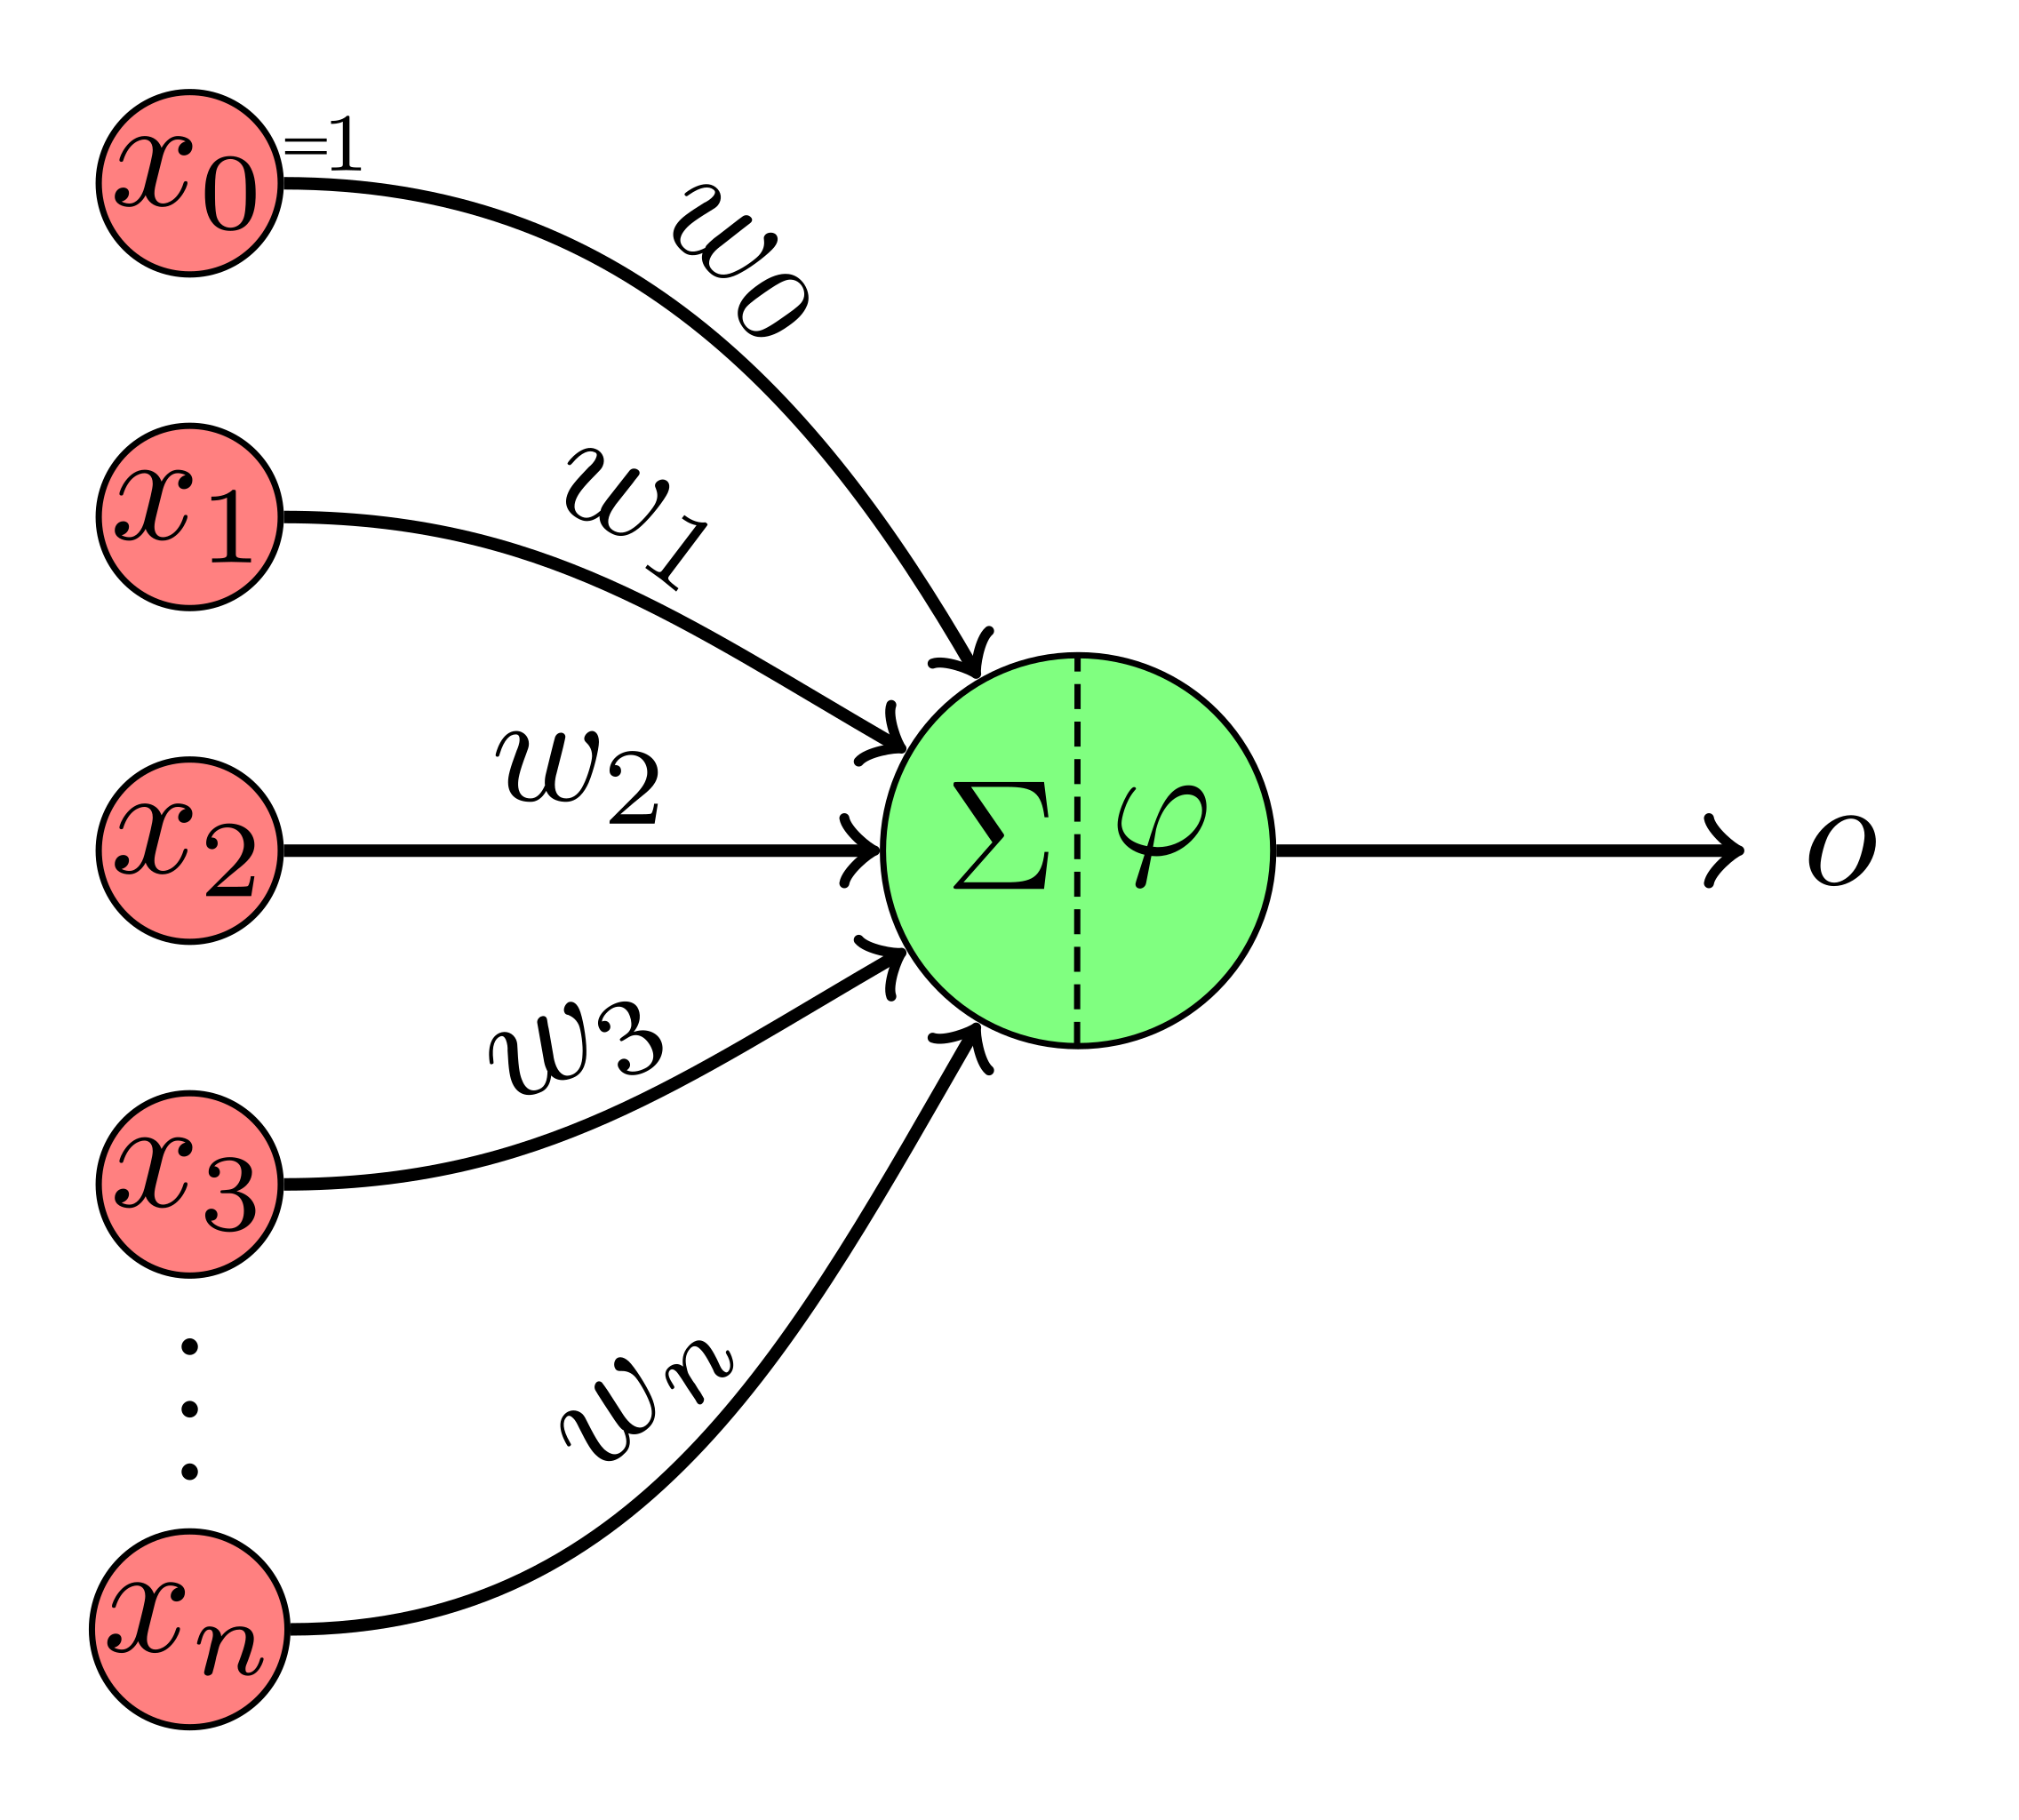
\includegraphics[width=0.5\textwidth]{figures/perceptron.png}
  \end{center}
  \caption{Model of a perceptron. The inputs xi-n are multiplied with their corresponding weights wi-n, summed up and fed to the transfer function (in the figure denoted as phi). Finally, an output value o is produced. Bias is omitted in this figure.}
  \label{fig:perceptron}
\end{figure}

Perceptrons can be stacked after and next to one another (in the latter case known as a layer), called a multi-layer perceptron (MLP). The first layer, where the input signal is the input data itself, represented in floating point numbers, is called the input layer. The last layer, where the output signal corresponds to the decision or classification, is called the output layer. Any layer between the input layer and the output layer is called a hidden layer. Together these layers form what is known as an Artificial Neural Network (ANN). Any ANN with at least two hidden layers is called a Deep Neural Network (DNN).

I used Figure \ref{fig:perceptron} above and referred to it.


\section{Training a Deep Neural Network}

Neural networks can learn to approximate functions through learning. Learning occurs by updating the weights and biases of the perceptrons gradually to approximate the desired output value of the last layer in the neural network. This difference between the desired output value and the output of the network, also known as the cross-entropy, is estimated by using a cost function.  

\textbf{TODO formula}
By updating the weights according to a paradigm, the cost can be minimized. A gradient-based approach to minimizing the cost is called backpropagation. Backpropagation is defined as taking the following steps:
\begin{enumerate}
\item Forward the input through the neural network to generate a prediction yhat.
\item Measure the cross-entropy loss e.g. according to Formula X.2
\item Propagate back the error’s gradient from the last(output) to the first(input) layer of the network.
\item Change the weights and biases based on the gradient.
\end{enumerate}

\textbf{TODO formula}

where wj is the weights of the DNN and yhat can be seen as a non-linear function of the weights.  

\textbf{TODO formula}

\section{Challenges in training}

In real world applications, there are many challenges when training a deep neural network.

\subsection{Overfitting/underfitting}

With a large number of parameters, the network can be said to have a high degree of freedom. It becomes so complex that it will encounter the overfitting problem [Source]. Overfitting means that the network will tend towards having lower accuracy of the test dataset, despite an increasing accuracy on the training dataset. This phenomenon can be anecdotally compared to memorizing the training dataset by heart, and thus losing the generalization property when tested on data outside the training dataset. 

Several approaches can be taken to minimize or resolve the problem of overfitting.
\begin{enumerate}
\item Regularization [Source, 19]: By imposing a cost (or penalty) on the optimization function, the optimal solution can be made unique.
\item Early stopping [Source, 20]: By halting the training when the error of the test dataset reaches its minimum, overfitting can be avoided. Early stopping can be thought of as regularization in the temporal domain. 
\item Dropout [Source, 21]: By randomly ignoring some neurons during training to reduce the model complexity, an increase in model sparsity is gained. 
\item Data augmentation [Source, 22]: Additional data is created, typically in preprocessing, by altering the original data in a number of ways which are added in addition to the original data. For visual data, some examples are: changing angles, illumination, saturation, exposure, etc. This creates additional variance which prevents simply memorizing shallow features in the dataset.
\end{enumerate}

\subsection{Exploding/vanishing gradients}
When the backpropagation algorithm backflows the error gradient from the output layer back towards the input layer, the gradient will diminish by the layer if the initial gradient is smaller than 1.0, and increase substantially when initially greater than 1.0. As a result, some parameters will either remain unchanged by the diminished gradient or changed by a very large value by the time the update process reaches very deep in large networks.

Some techniques for overcoming the exploding/vanishing gradient [Source] problem are:

\begin{enumerate}
\item Non-saturating activation functions: Using e.g. ReLU [Source] instead of the commonly used sigmoid activation function can help during training. The gradient is minimal when the sigmoid function is close to its output limits (-1/1) meaning it will saturate. Using ReLU = max(0,z) won't have this problem. However, ReLU has its own problem in that some perceptrons may stop outputting values except for 0. This is known as the dying ReLU problem. The solution is to use leaky ReLU = max(az,z) where a is the slope when z < 0. 

\item TODO visualization

\item Gradient clipping [Source]: Clipping the gradient by defining a max value it can attain during backpropagation means it will never exceed a certain threshold. This solves the exploding gradient problem.

\item Batch Normalization [Source]: A technique used to address the problem that the distribution of each layer’s inputs changes during training, as the parameters of the previous layers change, by zero centering the input, scaling and then shifting the result. TODO two formulas

\end{enumerate}
\subsection{Improving gradient descent}

Training speed can be improved by using techniques to update the learning rate during training, making the model converge faster towards the desired weight distribution.
\begin{enumerate}
\item Momentum: TODO
\item Weight decay: TODO
\end{enumerate}


\section{Convolutional Neural Network}

\cleardoublepage
\chapter{Method or Methods}
\label{ch:methods}
\todo[inline, backgroundcolor=kth-lightblue]{Metod eller Metodval}
\todo[inline]{This chapter is about Engineering-related
  content, Methodologies and Methods.  Use a self-explaining title.\\The
  contents and structure of this chapter will change with your choice of
  methodology and methods.}



\todo[inline]{Describe the engineering-related contents (preferably with models) and the research methodology and methods that are used in the degree project.\\
Give a theoretical description of the scientific or engineering methodology are you going to use and why have you chosen this method. What other methods did you consider and why did you reject them.\\
In this chapter, you describe what engineering-related and scientific skills you are going to apply, such as modeling, analyzing, developing, and evaluating engineering-related and scientific content. The choice of these methods should be appropriate for the problem . Additionally, you should be consciousness of aspects relating to society and ethics (if applicable). The choices should also reflect your goals and what you (or someone else) should be able to do as a result of your solution - which could not be done well before you started.}

The purpose of this chapter is to provide an overview of the research method
used in this thesis. Section~\ref{sec:researchProcess} describes the research
process. Section~\ref{sec:researchParadigm} details the research
paradigm. Section~\ref{sec:dataCollection} focuses on the data collection
techniques used for this research. Section~\ref{sec:experimentalDesign}
describes the experimental design. Section~\ref{sec:assessingReliability}
explains the techniques used to evaluate the reliability and validity of the
data collected. Section~\ref{sec:plannedDataAnalysis} describes the method
used for the data analysis. Finally, Section~\ref{sec:evaluationFramework}
describes the framework selected to evaluate xxx.

\todo[inline, backgroundcolor=kth-lightblue]{Vilka vetenskapliga eller ingenjörsmetodik ska du använda och varför har du valt den här metoden. Vilka andra metoder gjorde du överväga och varför du avvisar dem.
Vad är dina mål? (Vad ska du kunna göra som ett resultat av din lösning - vilken inte kan göras i god tid innan du började)
Vad du ska göra? Hur? Varför? Till exempel, om du har implementerat en artefakt vad gjorde du och varför? Hur kommer ditt utvärdera den.
Syftet med detta kapitel är att ge en översikt över forsknings metod som
används i denna avhandling. Avsnitt~\ref{sec:researchProcess} beskriver forskningsprocessen. Avsnitt~\ref{sec:researchParadigm} detaljer forskningen paradigm. Avsnitt~\ref{sec:dataCollection} fokuserar på datainsamling
tekniker som används för denna forskning. Avsnitt~\ref{sec:experimentalDesign} beskriver experimentell
design. Avsnitt~\ref{sec:assessingReliability} förklarar de tekniker som används för att utvärdera
tillförlitligheten och giltigheten av de insamlade uppgifterna. Avsnitt~\ref{sec:plannedDataAnalysis}
beskriver den metod som används för dataanalysen. Slutligen, Avsnitt~\ref{sec:evaluationFramework}
beskriver ramverket valts för att utvärdera xxx.\\
Ofta kan man koppla ett antal följdfrågor till undersökningsfrågan och problemlösningen t ex\\
(1) Vilken process skall användas för konstruktion av lösningen och vilken process skall kopplas till denna för att svara på undersökningsfrågan?\\
(2) Hur och vilket resultat (storheter) skall presenteras både för att redovisa svar på undersökningsfrågan (resultatkapitlet i denna rapport) och redovisa resultat av problemlösningen (prototypen, ofta dokument som bilagor men vilka dokument och varför?).\\
(3) Vilken teori/teknik skall väljas och användas både för undersökningen (taxonomi, matematik, grafer, storheter mm)  och  problemlösning (UML, UseCases, Java mm) och varför?\\
(4) Vad behöver du som student leverera för att uppnå hög kvaliet (minimikrav) eller mycket hög kvalitet på examensarbetet?\\
(5) Frågorna kopplar till de följande underkapitlen.\\
(6) Resonemanget bygger på att studenter på hing-programmet ofta skall konstruera något åt problemägaren och att man till detta måste koppla en intressant ingenjörsfråga. Det finns hela tiden en dualism mellan dessa aspekter i exjobbet.
}

\section{Research Process}
\label{sec:researchProcess}
\todo[inline, backgroundcolor=kth-lightblue]{Undersökningsrocess och utvecklingsprocess}

Figure~\ref{fig:researchprocess} shows the steps conducted in order to carry out this research. 

\todo[inline, backgroundcolor=kth-lightblue]{Figur~\ref{fig:researchprocess} visar de steg som utförs för att genomföra\\
Beskriv, gärna med ett aktivitetsdiagram (UML?), din undersökningsprocess och utvecklingsprocess.  Du måste koppla ihop det akademiska intresset (undersökningsprocess) med ursprungsproblemet (utvecklingsprocess)
denna forskning.\\
Aktivitetsdiagram från t ex UML-standard}


 
\begin{figure}[!ht]
  \begin{center}
    
\includegraphics[width=0.5\textwidth]{figures/researchprocess.png}
  \end{center}
  \caption{Research Process}
  \label{fig:researchprocess}
\end{figure}
\todo[inline, backgroundcolor=kth-lightblue]{Forskningsprocessen}

\section{Research Paradigm}
\label{sec:researchParadigm}
\todo[inline, backgroundcolor=kth-lightblue]{Undersökningsparadigm\\
Exempelvis\\
Positivistisk (vad/hur fungerar det?) kvalitativ fallstudie med en deduktivt (förbestämd) vald ansats och ett induktivt(efterhand uppstår dataområden och data) insamlade av data och erfarenheter.}


\section{Data Collection}
\label{sec:dataCollection}
\todo[inline]{This should also show that you are aware of the social and ethical concerns that might be relevant to your data collection method.)}

\todo[inline, backgroundcolor=kth-lightblue]{Datainsamling\\
(Detta bör också visa att du är medveten om de sociala och etiska frågor som
kan vara relevanta för dina data insamlingsmetod.)}

\subsection{Sampling}
\todo[inline, backgroundcolor=kth-lightblue]{Stickprovsundersökning}

\subsection{Sample Size}
\todo[inline, backgroundcolor=kth-lightblue]{Provstorleken}

\subsection{Target Population}
\todo[inline, backgroundcolor=kth-lightblue]{Målgruppen}

\section{Experimental design/Planned Measurements}
\label{sec:experimentalDesign}
\todo[inline, backgroundcolor=kth-lightblue]{Experimentdesign/Mätuppställning}

\subsection{Test environment/test bed/model}\todo[inline]{Describe everything that someone else would need to reproduce your test environment/test bed/model/… .}
\todo[inline, backgroundcolor=kth-lightblue]{Testmiljö/testbädd/modell\\
Beskriv allt att någon annan skulle behöva återskapa din testmiljö / testbädd / modell / …}

\subsection{Hardware/Software to be used}
\todo[inline, backgroundcolor=kth-lightblue]{Hårdvara / programvara som ska användas}


\section{Assessing reliability and validity of the data collected}
\label{sec:assessingReliability}
\todo[inline, backgroundcolor=kth-lightblue]{Bedömning av validitet och reliabilitet hos använda metoder och insamlade data }


\subsection{Validity of method}
\label{sec:validtyOfMethod}
\todo[inline]{How will you know if your results are valid?}
\todo[inline, backgroundcolor=kth-lightblue]{Giltigheten av metoder\\
  Har dina metoder ge dig de rätta svaren och lösning? Var metoderna korrekt?}

\subsection{Reliability of method}
\label{sec:reliabilityOfMethod}
\todo[inline]{How will you know if your results are reliable?}
\todo[inline, backgroundcolor=kth-lightblue]{Tillförlitlighet av metoder\\
Hur bra är dina metoder, finns det bättre metoder? Hur kan du förbättra dem?}

\subsection{Data validity}
\label{sec:dataValidity}
\todo[inline, backgroundcolor=kth-lightblue]{Giltigheten av uppgifter\\
Hur vet du om dina resultat är giltiga? Har ditt resultat mäta rätta?}

\subsection{Reliability of data}
\label{sec:reliabilityOfData}
\todo[inline, backgroundcolor=kth-lightblue]{Tillförlitlighet av data\\
Hur vet du om dina resultat är tillförlitliga? Hur bra är dina resultat?}


\section{Planned Data Analysis}
\label{sec:plannedDataAnalysis}
\todo[inline, backgroundcolor=kth-lightblue]{Metod för analys av data}


\subsection{Data Analysis Technique}
\label{sec:dataAnalysisTechnique}
\todo[inline, backgroundcolor=kth-lightblue]{Dataanalys Teknik}

\subsection{Software Tools}
\label{sec:softwareTools}
\todo[inline, backgroundcolor=kth-lightblue]{Mjukvaruverktyg}


\section{Evaluation framework}
\label{sec:evaluationFramework}
\todo[inline, backgroundcolor=kth-lightblue]{Utvärdering och ramverk\\
Metod för utvärdering, jämförelse mm. Kopplar till kapitel~\ref{ch:resultsAndAnalysis}.}

\section{System documentation}\todo[inline]{If this is going to be a complete document consider putting it in as an appendix, then just put the highlights here.}
\todo[inline, backgroundcolor=kth-lightblue]{Systemdokumentation\\
Med vilka dokument och hur skall en konstruerad prototyp dokumenteras? Detta blir ofta bilagor till rapporten och det som problemägaren till det ursprungliga problemet (industrin) ofta vill ha.\\
Bland dessa bilagor återfinns ofta, och enligt någon angiven standard, kravdokument, arkitekturdokument, designdokumnet, implementationsdokument, driftsdokument, testprotokoll mm.}

\cleardoublepage
\chapter{What you did}\todo[inline]{Choose your own chapter title to describe this}
\label{ch:whatYouDid}
\todo[inline, backgroundcolor=kth-lightblue]{[Vad gjorde du? Hur gick det till? – Välj lämplig rubrik (“Genomförande”, “Konstruktion”, ”Utveckling”  eller annat]}


\todo[inline]{What have you done? How did you do it? What design decisions did you make? How did what you did help you to meet your goals?}
\todo[inline, backgroundcolor=kth-lightblue]{Vad du har gjort? Hur gjorde du det? Vad designen beslut gjorde du?\\
Hur kom det du hjälpte dig att uppnå dina mål?}

% the following sets the TOC entry to break after the & - note you have to include the first letter of the following word as it get swolled by the \texorpdfstring{}{} processing
\section[Hardware/Software design …/Model/Simulation model \&\texorpdfstring{\\}{ p} parameters/…]{Hardware/Software design …/Model/Simulation model \& parameters/…}
\todo[inline, backgroundcolor=kth-lightblue]{Hårdvara / Mjukvarudesign ... / modell / Simuleringsmodell och parametrar / …}

Figure~\ref{fig:homepageicon} shows a simple icon for a home page. The time
to access this page when served will be quantified in a series of
experiments. The configurations that have been tested in the test bed are
listed in Table~\ref{tab:configstested}.

\todo[inline, backgroundcolor=kth-lightblue]{Figur~\ref{fig:homepageicon}  visar en enkel ikon för en hemsida. Tiden för att få tillgång till den här sidan när serveras kommer att kvantifieras i en serie experiment. De konfigurationer som har testats i provbänk listas ini tabell~\ref{tab:configstested}.\\
Vad du har gjort? Hur gjorde du det? Vad designen beslut gjorde du?}
 
\begin{figure}[!ht]
  \begin{center}
    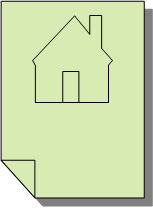
\includegraphics[width=0.25\textwidth]{figures/Homepage-icon.png}
  \end{center}
  \caption{Homepage icon}
  \label{fig:homepageicon}
\end{figure}

\begin{table}[!ht]
  \begin{center}
    \caption{Configurations tested}
    \label{tab:configstested}
    \begin{tabular}{l|c} % <-- Alignments: 1st column left, 2nd middle and 3rd right, with vertical lines in between
      \textbf{Configuration} & \textbf{Description} \\
      \hline
      1 & Simple test with one server\\
      2 & Simple test with one server\\
    \end{tabular}
  \end{center}
\end{table}
\todo[inline, backgroundcolor=kth-lightblue]{Konfigurationer testade}

\section{Implementation …/Modeling/Simulation/…}
\label{sec:implementationDetails}
\todo[inline, backgroundcolor=kth-lightblue]{Implementering … / modellering / simulering / …}


\subsection{Some examples of coding}

Listing~\ref{lst:helloWorldInC} shows an example of a simple program written
in C code.

\begin{lstlisting}[language={C}, caption={Hello world in C code}, label=lst:helloWorldInC]
int main() {
printf("hello, world");
return 0;
}
\end{lstlisting}


In contrast, Listing~\ref{lst:programmes} is an example of code in Python to
get a list of all of the programs at KTH.

\lstset{extendedchars=true}
\begin{lstlisting}[language={Python}, caption={Using a python program to
    access the KTH API to get all of the programs at KTH}, label=lst:programmes]
KOPPSbaseUrl = 'https://www.kth.se'

def v1_get_programmes():
    global Verbose_Flag
    #
    # Use the KOPPS API to get the data
    # note that this returns XML
    url = "{0}/api/kopps/v1/programme".format(KOPPSbaseUrl)
    if Verbose_Flag:
        print("url: " + url)
    #
    r = requests.get(url)
    if Verbose_Flag:
        print("result of getting v1 programme: {}".format(r.text))
    #
    if r.status_code == requests.codes.ok:
        return r.text           # simply return the XML
    #
    return None
\end{lstlisting}


\cleardoublepage
\chapter{Results and Analysis}
\label{ch:resultsAndAnalysis}
\todo[inline, backgroundcolor=kth-lightblue]{svensk: Resultat och Analys}

\todo[inline]{
Sometimes this is split into two chapters.\\
  
Keep in mind: How you are going to evaluate what you have done? What are your metrics?\\
Analysis of your data and proposed solution\\
Does this meet the goals which you had when you started?
}

In this chapter, we present the results and discuss them.

\todo[inline, backgroundcolor=kth-lightblue]{I detta kapitel presenterar vi resultatet och diskutera dem.\\
Ibland delas detta upp i två kapitel.\\
Hur du ska utvärdera vad du har gjort? Vad är din statistik?\\
Analys av data och föreslagen lösning\\
Innebär detta att uppnå de mål som du hade när du började?
}

\section{Major results}
\todo[inline, backgroundcolor=kth-lightblue]{Huvudsakliga resultat}

Some statistics of the delay measurements are shown in Table~\ref{tab:delayMeasurements}.
The delay has been computed from the time the GET request is received until the response is sent.

\todo[inline, backgroundcolor=kth-lightblue]{Lite statistik av mätningarna fördröjnings visas i Tabell~\ref{tab:delayMeasurements}. Förseningen har beräknats från den tidpunkt då begäran GET tas emot fram till svaret skickas.}

\begin{table}[!ht]
  \begin{center}
    \caption{Delay measurement statistics}
    \label{tab:delayMeasurements}
    \begin{tabular}{l|S[table-format=4.2]|S[table-format=3.2]} % <-- Alignments: 1st column left, 2nd middle and 3rd right, with vertical lines in between
      \textbf{Configuration} & \textbf{Average delay (ns)} & \textbf{Median delay (ns)}\\
      \hline
      1 & 467.35 & 450.10\\
      2 & 1687.5 & 901.23\\
    \end{tabular}
  \end{center}
\end{table}
\todo[inline, backgroundcolor=kth-lightblue]{Fördröj mätstatistik}
\todo[inline, backgroundcolor=kth-lightblue]{Konfiguration | Genomsnittlig fördröjning (ns) | Median fördröjning (ns)}

Figure \ref{fig:processing_vs_payload_length} shows and example of the
performance as measured in the experiments.

\begin{figure}[!ht]
% GNUPLOT: LaTeX picture
\setlength{\unitlength}{0.240900pt}
\ifx\plotpoint\undefined\newsavebox{\plotpoint}\fi
\begin{picture}(1500,900)(0,0)
\sbox{\plotpoint}{\rule[-0.200pt]{0.400pt}{0.400pt}}%
\put(171.0,131.0){\rule[-0.200pt]{4.818pt}{0.400pt}}
\put(151,131){\makebox(0,0)[r]{ 1.5}}
\put(1419.0,131.0){\rule[-0.200pt]{4.818pt}{0.400pt}}
\put(171.0,212.0){\rule[-0.200pt]{4.818pt}{0.400pt}}
\put(151,212){\makebox(0,0)[r]{ 2}}
\put(1419.0,212.0){\rule[-0.200pt]{4.818pt}{0.400pt}}
\put(171.0,292.0){\rule[-0.200pt]{4.818pt}{0.400pt}}
\put(151,292){\makebox(0,0)[r]{ 2.5}}
\put(1419.0,292.0){\rule[-0.200pt]{4.818pt}{0.400pt}}
\put(171.0,373.0){\rule[-0.200pt]{4.818pt}{0.400pt}}
\put(151,373){\makebox(0,0)[r]{ 3}}
\put(1419.0,373.0){\rule[-0.200pt]{4.818pt}{0.400pt}}
\put(171.0,454.0){\rule[-0.200pt]{4.818pt}{0.400pt}}
\put(151,454){\makebox(0,0)[r]{ 3.5}}
\put(1419.0,454.0){\rule[-0.200pt]{4.818pt}{0.400pt}}
\put(171.0,534.0){\rule[-0.200pt]{4.818pt}{0.400pt}}
\put(151,534){\makebox(0,0)[r]{ 4}}
\put(1419.0,534.0){\rule[-0.200pt]{4.818pt}{0.400pt}}
\put(171.0,615.0){\rule[-0.200pt]{4.818pt}{0.400pt}}
\put(151,615){\makebox(0,0)[r]{ 4.5}}
\put(1419.0,615.0){\rule[-0.200pt]{4.818pt}{0.400pt}}
\put(171.0,695.0){\rule[-0.200pt]{4.818pt}{0.400pt}}
\put(151,695){\makebox(0,0)[r]{ 5}}
\put(1419.0,695.0){\rule[-0.200pt]{4.818pt}{0.400pt}}
\put(171.0,776.0){\rule[-0.200pt]{4.818pt}{0.400pt}}
\put(151,776){\makebox(0,0)[r]{ 5.5}}
\put(1419.0,776.0){\rule[-0.200pt]{4.818pt}{0.400pt}}
\put(171.0,131.0){\rule[-0.200pt]{0.400pt}{4.818pt}}
\put(171,90){\makebox(0,0){ 0}}
\put(171.0,756.0){\rule[-0.200pt]{0.400pt}{4.818pt}}
\put(298.0,131.0){\rule[-0.200pt]{0.400pt}{4.818pt}}
\put(298,90){\makebox(0,0){ 10}}
\put(298.0,756.0){\rule[-0.200pt]{0.400pt}{4.818pt}}
\put(425.0,131.0){\rule[-0.200pt]{0.400pt}{4.818pt}}
\put(425,90){\makebox(0,0){ 20}}
\put(425.0,756.0){\rule[-0.200pt]{0.400pt}{4.818pt}}
\put(551.0,131.0){\rule[-0.200pt]{0.400pt}{4.818pt}}
\put(551,90){\makebox(0,0){ 30}}
\put(551.0,756.0){\rule[-0.200pt]{0.400pt}{4.818pt}}
\put(678.0,131.0){\rule[-0.200pt]{0.400pt}{4.818pt}}
\put(678,90){\makebox(0,0){ 40}}
\put(678.0,756.0){\rule[-0.200pt]{0.400pt}{4.818pt}}
\put(805.0,131.0){\rule[-0.200pt]{0.400pt}{4.818pt}}
\put(805,90){\makebox(0,0){ 50}}
\put(805.0,756.0){\rule[-0.200pt]{0.400pt}{4.818pt}}
\put(932.0,131.0){\rule[-0.200pt]{0.400pt}{4.818pt}}
\put(932,90){\makebox(0,0){ 60}}
\put(932.0,756.0){\rule[-0.200pt]{0.400pt}{4.818pt}}
\put(1059.0,131.0){\rule[-0.200pt]{0.400pt}{4.818pt}}
\put(1059,90){\makebox(0,0){ 70}}
\put(1059.0,756.0){\rule[-0.200pt]{0.400pt}{4.818pt}}
\put(1185.0,131.0){\rule[-0.200pt]{0.400pt}{4.818pt}}
\put(1185,90){\makebox(0,0){ 80}}
\put(1185.0,756.0){\rule[-0.200pt]{0.400pt}{4.818pt}}
\put(1312.0,131.0){\rule[-0.200pt]{0.400pt}{4.818pt}}
\put(1312,90){\makebox(0,0){ 90}}
\put(1312.0,756.0){\rule[-0.200pt]{0.400pt}{4.818pt}}
\put(1439.0,131.0){\rule[-0.200pt]{0.400pt}{4.818pt}}
\put(1439,90){\makebox(0,0){ 100}}
\put(1439.0,756.0){\rule[-0.200pt]{0.400pt}{4.818pt}}
\put(171.0,131.0){\rule[-0.200pt]{0.400pt}{155.380pt}}
\put(171.0,131.0){\rule[-0.200pt]{305.461pt}{0.400pt}}
\put(1439.0,131.0){\rule[-0.200pt]{0.400pt}{155.380pt}}
\put(171.0,776.0){\rule[-0.200pt]{305.461pt}{0.400pt}}
\put(30,453){\rotatebox{-270}{\makebox(0,0){Processing time (ms)}}}
\put(805,29){\makebox(0,0){Payload size (bytes)}}
\put(868.0,131.0){\rule[-0.200pt]{0.400pt}{84.074pt}}
\put(995.0,131.0){\rule[-0.200pt]{0.400pt}{98.287pt}}
\put(1173.0,131.0){\rule[-0.200pt]{0.400pt}{118.041pt}}
\put(1325.0,131.0){\rule[-0.200pt]{0.400pt}{134.904pt}}
\put(1350.0,131.0){\rule[-0.200pt]{0.400pt}{137.795pt}}
\put(1439.0,131.0){\rule[-0.200pt]{0.400pt}{155.380pt}}
\end{picture}
\caption[A GNUplot figure]{Processing time vs. payload length}\vspace{0.5cm}
\label{fig:processing_vs_payload_length}
\end{figure}
		

Given these measurements, we can calculate our processing bit rate as the inverse of the time it takes to process an additional byte divided by 8 bits per byte:

\[
	bitrate = \frac{1}{\frac{time_{byte}}{8}} = 20.03 \quad kb/s
\] 

\section{Reliability Analysis}
\todo[inline, backgroundcolor=kth-lightblue]{Analys av reabilitet\\
Reabilitet i metod och data}

\section{Validity Analysis}
\todo[inline, backgroundcolor=kth-lightblue]{Analys av validitet\\
Validitet i metod och data}

\cleardoublepage
\chapter{Discussion}\todo[inline]{This can be a separate chapter or a section
  in the previous chapter.}
\label{ch:discussion}
\todo[inline, backgroundcolor=kth-lightblue]{Diskussion\\
Förbättringsförslag?}

\cleardoublepage
\chapter{Conclusions and Future work}
\label{ch:conclusionsAndFutureWork}
\todo[inline, backgroundcolor=kth-lightblue]{Slutsats och framtida arbete}

\todo[inline]{Add text to introduce the subsections of this chapter.}

\section{Conclusions}
\label{sec:conclusions}
\todo[inline]{Describe the conclusions (reflect on the whole introduction given in Chapter 1).}
\todo[inline, backgroundcolor=kth-lightblue]{Slutsatser}

  
\todo[inline]{Discuss the positive effects and the drawbacks.\\
Describe the evaluation of the results of the degree project.\\
Did you meet your goals?\\
What insights have you gained?\\
What suggestions can you give to others working in this area?\\
If you had it to do again, what would you have done differently?}

\todo[inline, backgroundcolor=kth-lightblue]{Träffade du dina mål?\\
Vilka insikter har du fått?\\
Vilka förslag kan du ge till andra som arbetar inom detta område?
Om du hade att göra igen, vad skulle du ha gjort annorlunda?}

\section{Limitations}
\label{sec:limitations}
\todo[inline]{What did you find that limited your
  efforts? What are the limitations of your results?}
\todo[inline, backgroundcolor=kth-lightblue]{Begränsande faktorer\\
Vad gjorde du som begränsade dina ansträngningar? Vilka är begränsningarna i dina resultat?}

\section{Future work}
\label{sec:futureWork}
\todo[inline]{Describe valid future work that you or someone else could or should do.\\
Consider: What you have left undone? What are the next obvious things to be done? What hints can you give to the next person who is going to follow up on your work?
}
\todo[inline, backgroundcolor=kth-lightblue]{Vad du har kvar ogjort?\\
Vad är nästa självklara saker som ska göras?\\
Vad tips kan du ge till nästa person som kommer att följa upp på ditt arbete?
}


Due to the breadth of the problem, only some of the initial goals have been
met. In these section we will focus on some of the remaining issues that
should be addressed in future work. ...

\subsection{What has been left undone?}
\label{what-has-been-left-undone}

The prototype does not address the third requirment, i.e., a yearly
unavailability of less than 3 minutes, this remains an open problem. ...

\subsubsection{Cost analysis}

The current prototype works, but the performance from a cost perspective makes
this an impractical solution. Future work must reduce the cost of this
solution, to do so a cost analysis needs to first be done. ...

\subsubsection{Security}

A future research effort is needed to address the security holes that results
from using a self-signed certificate. Page filling text mass. Page filling
text mass. ...


\subsection{Next obvious things to be done}

In particular, the author of this thesis wishes to point out xxxxxx remains as
a problem to be solved. Solving this problem is the next thing that should be
done. ...

\section{Reflections}
\label{sec:reflections}
\todo[inline]{What are the relevant economic, social,
  environmental, and ethical aspects of your work?
}
\todo[inline, backgroundcolor=kth-lightblue]{Reflektioner}
\todo[inline, backgroundcolor=kth-lightblue]{Vilka är de relevanta ekonomiska, sociala, miljömässiga och etiska aspekter av ditt arbete?}


One of the most important results is the reduction in the amount of
energy required to process each packet while at the same time reducing the
time required to process each packet.

%The thesis contributes to the \gls{UN}\enspace\glspl{SDG} numbers 1 and 9 by
%xxxx. 




\noindent\rule{\textwidth}{0.4mm}
\todo[inline]{In the references, let Zotero or other tool fill this
  in for you. I suggest an extended version of the IEEE  style, to include
  URLs, DOIs, ISBNs, etc., to make it easier for your reader to find
  them. This will make life easier for your opponents and examiner. \\

  IEEE Editorial Style Manual: \url{https://www.ieee.org/content/dam/ieee-org/ieee/web/org/conferences/style_references_manual.pdf}
}
\todo[inline, backgroundcolor=kth-lightblue]{Låt Zotero eller annat verktyg fylla i det här för dig. Jag föreslår en utökad version av IEEE stil - att inkludera webbadresser, DOI, ISBN etc. - för att göra det lättare för läsaren att hitta dem. Detta kommer att göra livet lättare för dina motståndare och examinator.}

\cleardoublepage
% Print the bibliography (and make it appear in the table of contents)
\renewcommand{\bibname}{References}
\addcontentsline{toc}{chapter}{References}

\ifbiblatex
    %\typeout{Biblatex current language is \currentlang}
    \printbibliography[heading=bibintoc]
\else
    \bibliography{references}
\fi




\cleardoublepage
\appendix
\renewcommand{\chaptermark}[1]{\markboth{Appendix \thechapter\relax:\thinspace\relax#1}{}}
\chapter{Something Extra}
\todo[inline, backgroundcolor=kth-lightblue]{svensk: Extra Material som Bilaga}

\section{Just for testing KTH colors}
\ifdigitaloutput
    \textbf{You have selected to optimize for digital output}
\else
    \textbf{You have selected to optimize for print output}
\fi
\begin{itemize}[noitemsep]
    \item Primary color
    \begin{itemize}
    \item \textcolor{kth-blue}{kth-blue \ifdigitaloutput
    actually Deep sea
    \fi} {\color{kth-blue} \rule{0.3\linewidth}{1mm} }\\

    \item \textcolor{kth-blue80}{kth-blue80} {\color{kth-blue80} \rule{0.3\linewidth}{1mm} }\\
\end{itemize}

\item  Secondary colors
\begin{itemize}[noitemsep]
    \item \textcolor{kth-lightblue}{kth-lightblue \ifdigitaloutput
    actually Stratosphere
    \fi} {\color{kth-lightblue} \rule{0.3\linewidth}{1mm} }\\

    \item \textcolor{kth-lightred}{kth-lightred \ifdigitaloutput
    actually Fluorescence\fi} {\color{kth-lightred} \rule{0.3\linewidth}{1mm} }\\

    \item \textcolor{kth-lightred80}{kth-lightred80} {\color{kth-lightred80} \rule{0.3\linewidth}{1mm} }\\

    \item \textcolor{kth-lightgreen}{kth-lightgreen \ifdigitaloutput
    actually Front-lawn\fi} {\color{kth-lightgreen} \rule{0.3\linewidth}{1mm} }\\

    \item \textcolor{kth-coolgray}{kth-coolgray \ifdigitaloutput
    actually Office\fi} {\color{kth-coolgray} \rule{0.3\linewidth}{1mm} }\\

    \item \textcolor{kth-coolgray80}{kth-coolgray80} {\color{kth-coolgray80} \rule{0.3\linewidth}{1mm} }
\end{itemize}
\end{itemize}

\textcolor{black}{black} {\color{black} \rule{\linewidth}{1mm} }

%% The following label is necessary for computing the last page number of the body of the report to include in the "For DIVA" information
\label{pg:lastPageofMainmatter}

\clearpage
\fancyhead{}  % Do not use header on this extra page or pages
% TODO diva stuff
%\section*{For DIVA}
%\lstset{numbers=none} %% remove any list line numbering
%\divainfo{pg:lastPageofPreface}{pg:lastPageofMainmatter}
\end{document}
